\section{Waste Package Spacing Sensitivity Study}\label{sec:spacing}
The waste package spacing, $s$ of geologic repository concept effects the areal 
decay heat burden in the repository and has a strong effect on the thermal 
energy deposited per unit area in the medium. 

In the creation of the \gls{STC} database, the waste package spacing was varied 
across a number of values for each isotope, $i$, limiting 
radius $r_{calc}$, thermal diffusivity $\alpha_{th}$, and thermal conductivity $K_{th}$, considered.  By 
varying the waste package spacing of the repository model from $0.1-5 [m]$
this sensitivity analysis succeeds in capturing the domain of 
waste package spacings present in geologic repository concepts under 
consideration. 

\begin{figure}[htbp!]
\begin{center}
%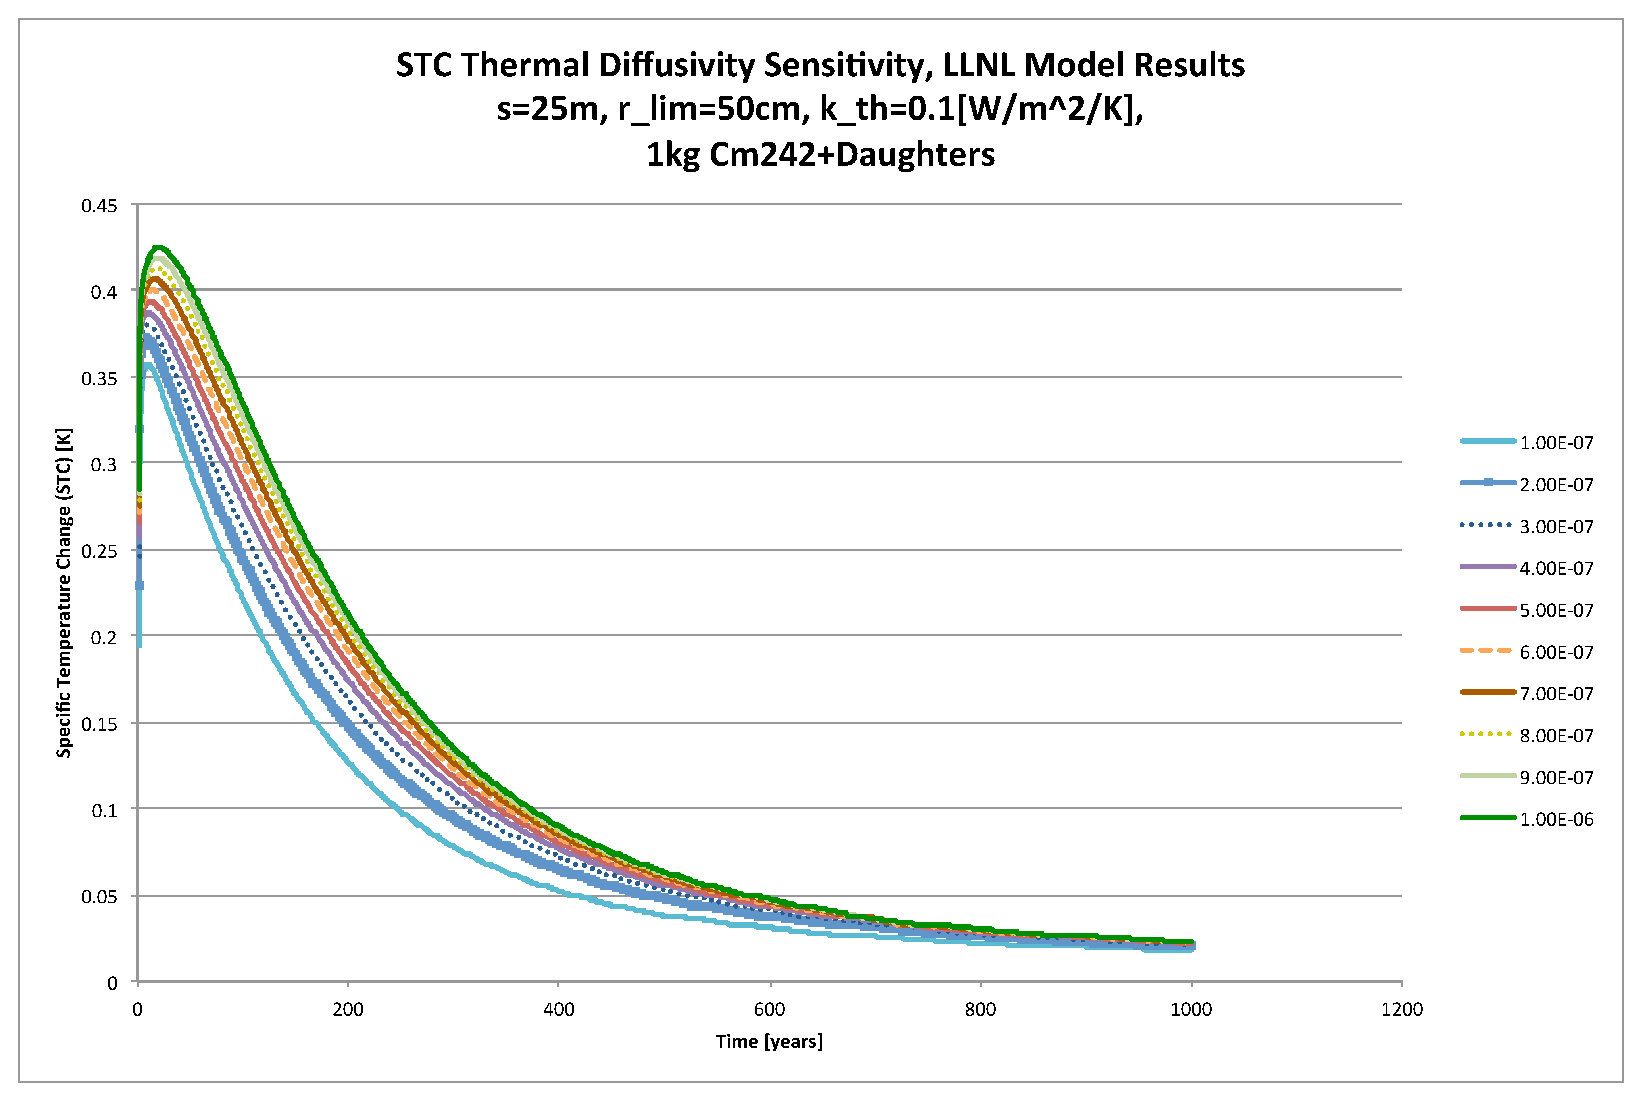
\includegraphics[width=0.7\textwidth]{./chapters/demonstration/diffusivity/Cm242alpha_kth_low.eps}
\end{center}
\caption[$K_{th}$ Sensitivity to $s$]{Increased waste package 
spacing decreases areal thermal energy deposition 
(here represented by \gls{STC}) in the near field (here $r_{calc} = 0.5m$).}
\label{fig:Cm242spacing}
\end{figure}

Figure \ref{fig:Cm242alpha_kth_low} shows the trend, visible for all isotopes, 
that increased waste package spacing of a medium decreases areal thermal energy 
deposition in the near field. This indicates that waste package spacing is 
an important parameter for repository concept design.

Similarly, the location of the limiting radius has a strong effect on the 
waste package loading limit, for a fixed limiting temperature. In Figure 
\ref{fig:Cm242r_lim}, the trend is demonstrated in which increased limiting 
radius decreases the thermal energy contributing to the thermal limit. 


\begin{figure}[htbp!]
\begin{center}
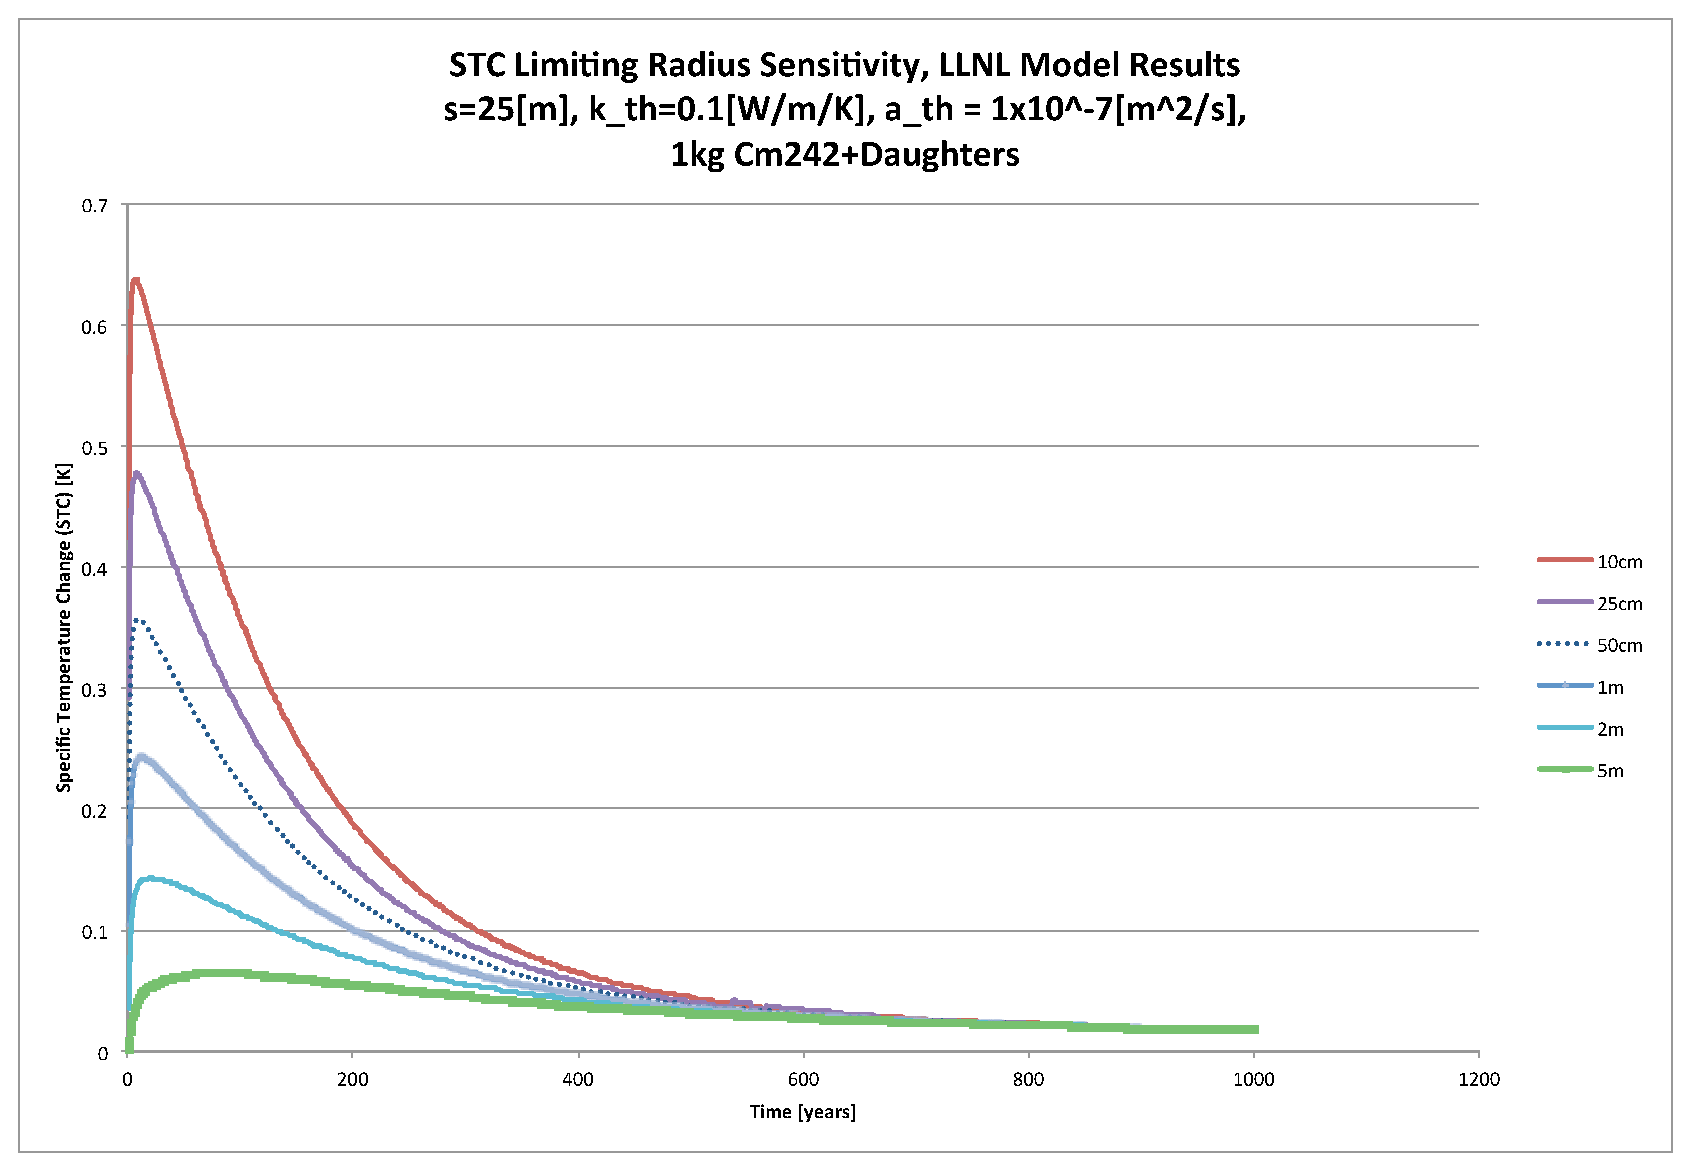
\includegraphics[width=0.7\textwidth]{./chapters/demonstration/diffusivity/Cm242r_lim_sens.eps}
\end{center}
\caption[$K_{th}$ Sensitivity to $r_{lim}$]{Increased limiting radius 
decreases thermal energy deposition contributing to the thermal limit
(here represented by \gls{STC}).}
\label{fig:Cm242r_lim_sens}
\end{figure}
